\documentclass[10pt,a4paper]{report}
\usepackage[latin1]{inputenc}
\usepackage{amsmath}
\usepackage{amsfonts}
\usepackage{color}
\usepackage{amssymb}
\usepackage{graphicx}
\usepackage{fancyhdr}
\lhead{Introduction to \\ Computer Graphics}
\chead{Exercise 1}
\rhead{Kevin Serrano, 204141 \\ Gianni Scarnera, 195899}
\pagestyle{fancy}
\author{Kevin Serrano, Gianni Scarnera}
\title{Exercise 1}
\begin{document}
\maketitle

\section*{Part 1}
\subsection*{Part 1.2 : Constant Shading}
We saw that the parameters of the function \textit{ConstantShader::shade} were a object \textit{IntersectionData} and a object \textit{Scene}. So in the constructor \textit{IntersectionData} we found the properties of the colour of the intersection. So we just take it and return the colour on the function \textit{ConstantShader::shade} to obtain the result display.
\begin{figure}[h!]
\caption{The result of part 1.2}
  \centering
    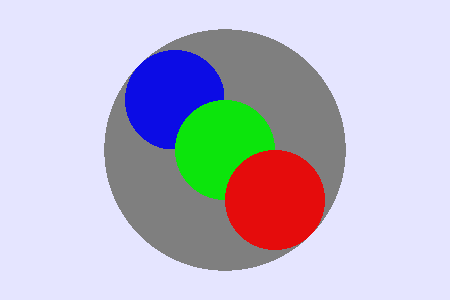
\includegraphics[width=1\textwidth]{framework/Image1_2.png}
\end{figure}
\newpage
\subsection*{Part 1.3}
We have to replace the orthographic camera with a perspective one. To do so, we first have to calculate the correct pixel length. Pixel length is a function of the opening angle and the resolution, namely tan(opening angle in rad divided by half the resolution ).

\begin{figure}[h!]
\caption{SimpleCamera model}
  \centering
    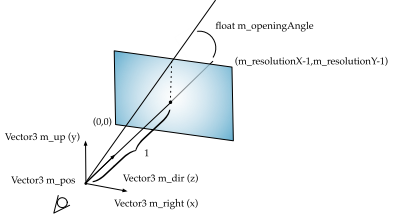
\includegraphics[width=0.7\textwidth]{pixelLength.png}
\end{figure}
 Furthermore, the position of the camera is now a single point and the direction of the rays are from the camera to each of the pixels on the screen multiplied by the camToWorld matrix.
\begin{figure}[h!]
\caption{The result of part 1.3}
  \centering
    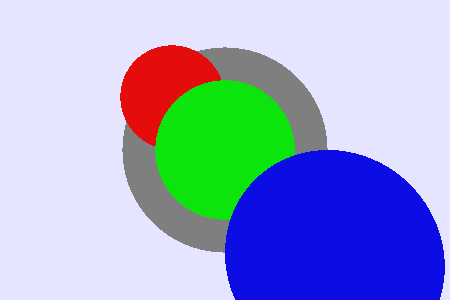
\includegraphics[width=1\textwidth]{framework/Image1_3.png}
\end{figure}
\newpage
\subsection*{Part 1.4.1 : class Plane}
To found the intersection for a plane, we have to resolve the equation $$(\bf{x}-\bf{p}) \cdot{\bf{n}} = 0$$ where $\bf{x}$ is the point of interest, $\bf p$ the point on plane and $\bf n$ the normal vector of the plane.
\begin{figure}[h!]
\caption{Plane intersection}
  \centering
    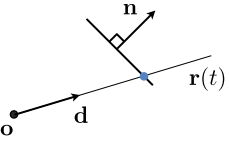
\includegraphics[width=0.3\textwidth]{planeIntersec.png}
\end{figure}
Then we can substitute the ray equation $\mathbf{o} + t\bf d$ (where $\bf o$ is the origin of the ray and $\bf d$ the direction of the ray) for $\bf x$ and solve for $t$. We get : $$ t = - {{(\bf o - \bf p) \cdot \bf n} \over {\bf d \cdot \bf n}}$$ and if ${\bf d \cdot \bf n = 0}$ then that means that the direction of the ray is parallel to te plane and then there is no intersection. So we have to do a test in the code to avoid a crash in compilation.

Then now we can return informations in the intersection by the object of type \textit{IntersectionData}, i.e it's position and it's color with the functions provided by the class \textit{IntersectionData}.
\begin{figure}[h!]
\caption{Plane intersection}
  \centering
    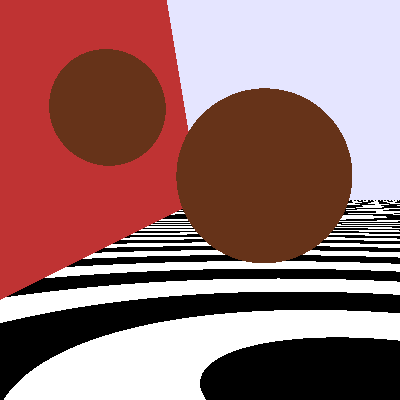
\includegraphics[width=0.5\textwidth]{Framework/Image1_4_1.png}
\end{figure}
\newpage
\subsection*{Part 1.4.2 : class Triangle}

To do this part, we can use the same technique as before except that now it more complicated to verify if the intersection is in the triangle. We used the first approach to resolve this problem, i.e intersect ray with triangle's plane.
First we use the barycentric coordinates $$ \mathbf{x} = s_1 \mathbf{p_1} + s_2 \mathbf{p_2} + s_3 \mathbf{p_3}$$ where $s_1, s_2, s_3$ are the tree area and $\bf p_1, p_2, p_3$ the three vertices of the triangles. Finally $\bf x$ is a point inside the triangle area and in our case it will be the ray intersection.

\begin{figure}[h!]
\caption{Barycentric coordinates of a triangle}
  \centering
    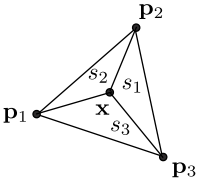
\includegraphics[width=0.3\textwidth]{triangle.png}
\end{figure}

So the ray intersection with the triangle is given by the following equation $$ (\mathbf{o} + t \mathbf{d} - \mathbf{p_1}) \cdot \mathbf{n} = 0$$ where $\bf n$ is the triangle's normal : $$\mathbf{n} = (\bf p_3 - p_1) \times (p_2 - p_1)$$ and then we can resolve for t : $$ t = - {{(\bf o - \bf p_1) \cdot \bf n} \over {\bf d \cdot \bf n}}$$
Again if ${\bf d \cdot \bf n = 0}$ then there are no solutions.

Now we can compute the three area $s_1, s_2, s_3$. To do that we created three vectors $\bf n_{s_1}, n_{s_2}, n_{s_3}$ wich are normal vector of the area $s_1, s_2, s_3$ respectively. So
\begin{itemize}
\item $\bf n_{s_1}$ is normal to the triangle of surface $s_1$. Then $\bf n_{s_1} = (\bf p_2-p_3) \times (x - p_3)$
\item $\bf n_{s_2}$ is normal to the triangle of surface $s_2$. Then $\bf n_{s_2} = (\bf p_1-p_2) \times (x - p_2)$
\item $\bf n_{s_3}$ is normal to the triangle of surface $s_3$. Then $\bf n_{s_3} = (\bf p_3-p_1) \times (x - p_1)$
\end{itemize}
where $\bf x$ is the intersection, given in the code by \textit{ray.getPointOnray(t)} with $t$ as above.
Now we have to normalise $s_1, s_2, s_3$ and verify if 
\begin{itemize}
\item $s_1 + s_2 + s_3 = 1$
\item $0 \leq s_i \leq 1$
\end{itemize}
and if it is ok, then that means that the intersection $\bf x$ is in the triangle and we have ton return the value of the object \textit{iData}.
To normalise $s_1, s_2, s_3$, we have the following formula $$s_i = \frac{\mathbf{n}\cdot \mathbf{n_{s_i}}}{||\mathbf{n}||^2}$$
\newpage
Then we obtain the result display in the figure below.
\begin{figure}[h!]
\caption{Triangle intersection}
  \centering
    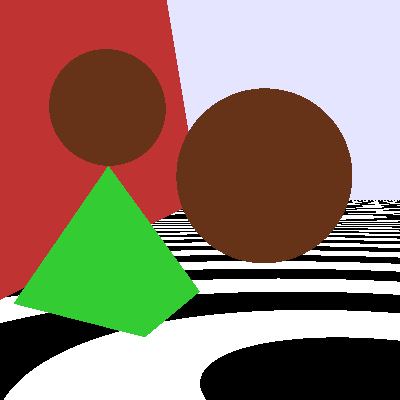
\includegraphics[width=0.5\textwidth]{Framework/Image1_4_2.png}
\end{figure}
\end{document}